En primera instancia escogimos `tipo de publicación' como shard key. Obtuvimos una distribución pareja, ya que eran 3 shards
para 3 rangos posibles. A simple vista podría parecer una buena clave, pero hay que tener en cuenta que los datos reales
podrían tener otra distribución, y la baja cardinalidad en ese caso sería un problema, suponiendo un 90\% de publicaciones de artículos 
implicaría tener los shards totalmente desbalanceados.

\begin{figure}[h!]
 \centering
 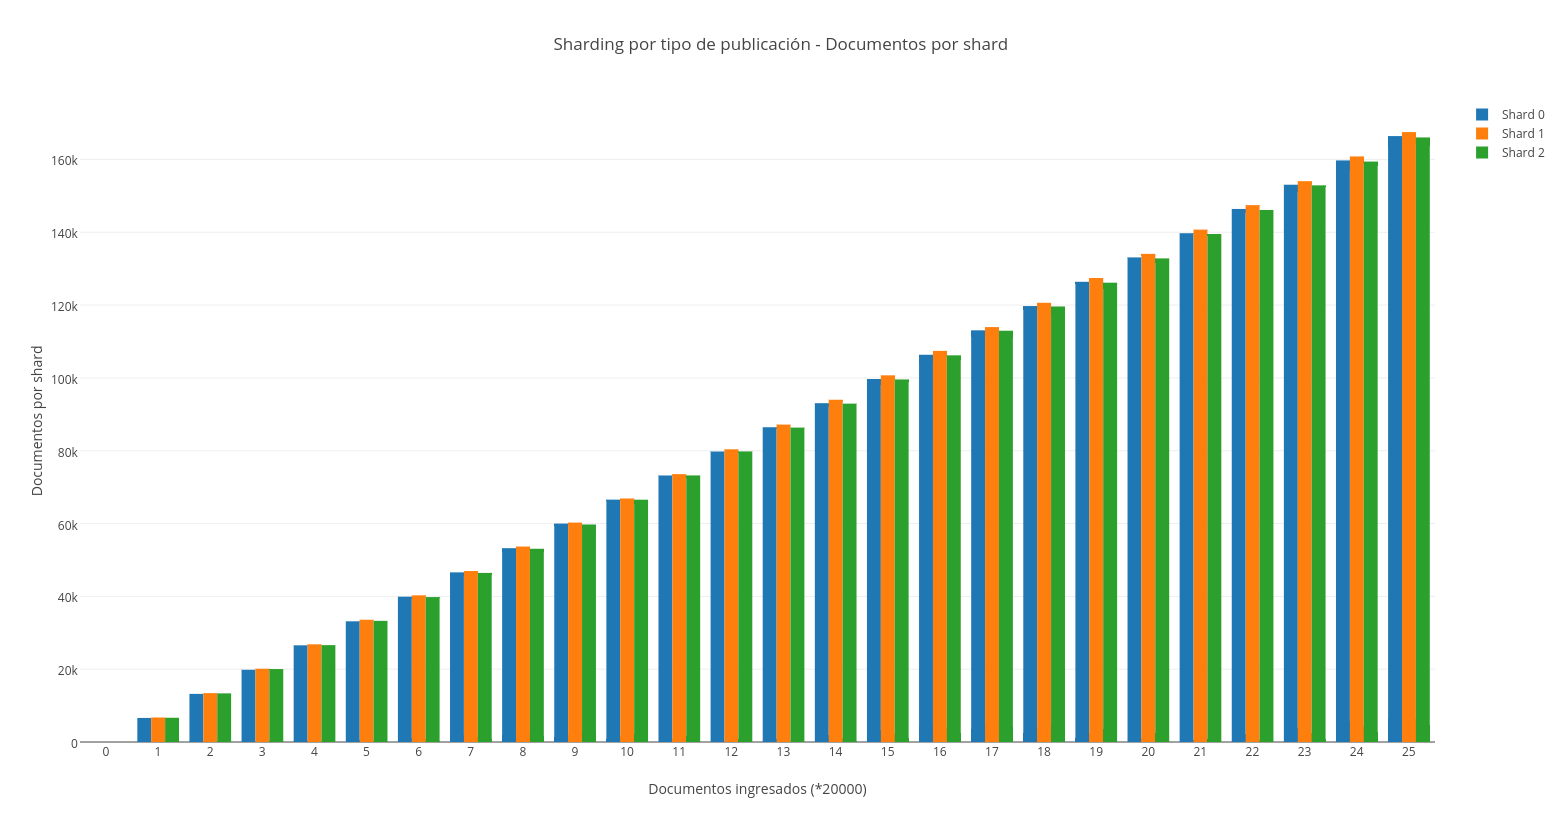
\includegraphics[scale=0.3,keepaspectratio=true]{./ShardingPorTipoDePublicacion-DocumentosPorShard.png}
 \caption{Documentos por Shard}
\end{figure}
 
Con los datos obtenidos a través de las pruebas, generamos gráficos a partir de otros parámetros como datos estimados por chunk y datos por shard, los omitimos en el
informe porque no agregan información interesante.

Para observar mejor el gráfico se puede acceder mediante el siguiente link a su representación online:
\begin{itemize}
 \item \href{https://plot.ly/~fzanollo/13/sharding-por-tipo-de-publicacion-documentos-por-shard/}{Documentos por shard}
\end{itemize}